% Intended LaTeX compiler: pdflatex
\documentclass{scrartcl}
    \usepackage{amsmath, amssymb, bm}
		\usepackage[utf8]{inputenc}
		\usepackage[dvipdfmx]{graphicx}
		\usepackage[dvipdfmx]{color}
		\usepackage[backend=biber,bibencoding=utf8]{biblatex}
		\usepackage{url}
		\usepackage{indentfirst}
		\usepackage[normalem]{ulem}
		\usepackage{longtable}
		\usepackage{minted}
		\usepackage{fancyvrb}
    \usepackage[dvipdfmx,colorlinks=false,pdfborder={0 0 0}]{hyperref}
    \usepackage{pxjahyper}
    \usepackage{caption}
\author{情報科学類3年 江畑 拓哉 (201611350)}
\date{}
\title{ヒューマンインタフェース演習課題3}
\begin{document}

\maketitle
\tableofcontents

\section{摂氏温度と華氏温度を変換するGUIアプリケーションを設計&実装せよ。}
\label{sec:org1b953a8}
 以下のレポジトリ [[\url{https://github.com/MokkeMeguru/clj-text-input} に成果物を置いた。利用方法はレポジトリの README.md にある。\\
 ソースコードは編集した部分のみを示す。\\
\subsection{設計}
\label{sec:org3b69e7c}
 入力を行いエンターキーを押すことで結果が表示できるようにすることで操作時間を短縮させようと考えた。また、Tabキーで入力枠を変更することでマウス操作を0にした。\\

\newpage\\
\subsection{clj-text-input/src/cljs/clj\_text\_input/core.cljs}
\label{sec:orgef27046}



\begin{minted}[frame=lines,linenos=true,obeytabs,tabsize=4]{clojure}
(defn form-input [label placeholder id fields start-time result]
  [:div.container
   [:div.form-group.flex.my-auto
    [:label label]
    [:input.form-control.input-lg ;; フォーム
     {:type :text
      :placeholder placeholder
      :value (id @fields)
      :on-change #(do ;; 入力を反映
                    (swap! fields assoc id (-> % .-target .-value)))
      :on-key-press (fn [e] ;; Enter キーを押されれば、計算を行い実行時間と共に表示する
                      (when (= 13 (.-charCode e))
                        (swap! result assoc :state true)
                        (swap! result assoc :t (- (.getTime (js/Date.)) @start-time))
                        (if (= id :cel)
                          (swap! result assoc
                                 :res
                                 (+ 32 (* 1.8 (id @fields))))
                          (swap! result assoc
                                 :res
                                 (/ (- (id @fields) 32) 1.8))))
                      (swap! fields {:cel nil :far nil}))}]]])

(defn res [result] ;; 結果を表示するための関数
  [:div.container
   (when (:state @result)
     [:div.flex.col
      [:label.col-md-4 "Result" [:p (:res @result)]]
      [:label.col-md-4 "Time" [:p (:t @result)]]])])

(defn home-page []
  [:div.container
   (let [fields (r/atom {:cel nil :far nil})
         start-time (r/atom nil)
         result (r/atom nil)]
     [:div.col
      [:button.btn.btn-primary.col-md-2 ;; 計測開始のためのボタン
       {:on-click #(do (reset! start-time (.getTime (js/Date.)))
                       (swap! result assoc :state false))}
       "Timer Start!"]
      [form-input "Celsius" "XX.X" :cel fields start-time result]
      [form-input "Fahrenheit" "XX.X" :far fields start-time result]
      [res result]
      ])])
\end{minted}

\subsection{スクリーンショット}
\label{sec:org53e496d}
\begin{center}
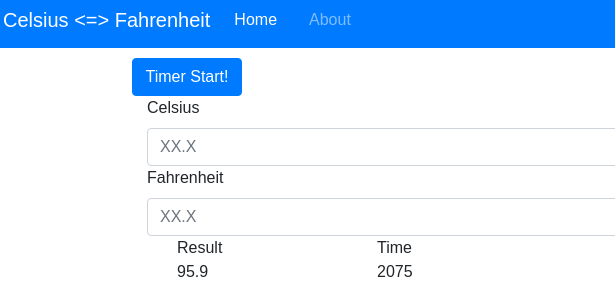
\includegraphics[width=0.9\linewidth]{./screen3.png}
\end{center}

\section{設計&実装したGUIにおいて、温度入力にどれだけ時間がかかるかを KLM に基づいて推定せよ。}
\label{sec:org655c47f}
\begin{itemize}
\item タイマーの開始ボタンをクリックする。(\(2\times B\))\\
\item タブキーを押して華氏温度か摂氏温度、いずれかの画面へ行く。(\((K + 2 \times K) / 2\))\\
\item 入力する温度を想起する。 (\(M\))\\
\item キーボードから XX.X と入力する。 (\(T(4)=4*K\))\\
\item エンターキーを押す。(\(T(1)=1\times K\))\\
\end{itemize}
\begin{equation*}
2\times B + 1.5 \times K + M + 4 \times K + K = 3.22(sec)
\end{equation*}
\section{設計&実装したGUIにおいて、温度の平均入力時間を、ユーザ実験して調べよ。}
\label{sec:orgb3f5f3b}
\begin{longtable}{|c|c|c||c|}
\hline
1回目 & 2回目 & 3回目 & 合計\\
\hline
\endfirsthead
\multicolumn{4}{l}{前ページからの続き} \\
\hline

1回目 & 2回目 & 3回目 & 合計 \\

\hline
\endhead
\hline\multicolumn{4}{r}{次ページに続く} \\
\endfoot
\endlastfoot
\hline
2942 & 2508 & 2685 & \\
2569 & 2292 & 2260 & \\
2819 & 2465 & 2871 & \\
4342 & 2214 & 3945 & \\
3796 & 2199 & 3219 & \\
2862 & 2200 & 2216 & \\
4114 & 2976 & 2891 & \\
2879 & 3242 & 2307 & \\
3013 & 3370 & 2740 & \\
3031 & 2750 & 2375 & \\
\hline
3236.7 & 2621.6 & 2750.9 & 2869.7333\\
\hline
\end{longtable}

\section{KLM による推測とユーザ実験の結果を比較して、考察せよ。}
\label{sec:org3ec9040}
 推測に比べてユーザ実験の結果がやや早いことがわかるが、一回目の10回測定の平均値は推測よりも遅いことがわかる。時間を置いたとしてもキーボード入力に慣れている学生を対象とした実験では、一旦この計測システム(入力システムとは別)にある程度慣れてしまえば、KLM による推測よりも多少早い結果になってしまうことは容易に想像できる。\\
 また、入力するキーの位置による問題も操作時間の短縮に寄与していると考えられる。今回数字の入力はテンキーを用いて行ったが、これはアルファベットが印字されている側のキーで数字を入力することに比べ指の移動距離が短く、また電卓の入力に慣れていれば更に反射的な入力が可能になってしまう。\\
 以上のことを考慮して実験結果を見つめ直せば、この実験結果は少なくとも KLM が示したい実行時間の見積もり手法を大きく外れるものではないと考えられる。\\
\end{document}
